
The jet images are used as input for a deep neural network classifier.
This section describes the implementation of the neural network and characterizes the properties and performance of the classifier.

\subsection{Network architecture and training}

In the studies presented in this note we make use of a deep convolutional neural network (CNN) to build a classifier of jet images.
CNNs are a class of deep, feed-forward artificial neural networks based on modular sets of weights (filters) that operate linearly on a small $m\times n$
patch of the input image. The output of each filter is the dot-product between the weights and the pixel in the corresponding patch and it is typically assigned the position of the
centre of the patch.
Each filter is then \emph{convolved} with the input image, by applying it to the whole image, a patch at a time, while moving the filter location across the image with a given stride.
As a result of this operation, a new output image is obtained for each filter used.
A non-linear activation function is typically applied to each pixel of the convolved image.
A down-sampling procedure, referred to as Max-pooling~\cite{MAXPOOL}, is then performed.
This procedure takes non-overlapping patches of convolution outputs as input, and outputs the maximum value for each patch.
The sets of filters, the activations and the Max-pooling constitute the fundamental building block for CNNs.
The depth of the network is determined by the number of convolutions concatenated in the network.

The CNN architecture used in this note follows the example of Ref.~\cite{Komiske:2016rsd} and consists of three iterations of a convolutional layer with a
Rectified Linear Unit (ReLU) activation~\cite{RELU} and paired with a Max-pooling layer,
all followed by a dense layer of 128 neurons with a ReLU activation. The output of the network is a softmax function~\cite{Goodfellow-et-al-2016-Book} of size two, 
predicting the probability for the quark jet and the gluon jet class, respectively. 
The convolutional layers consist of 128, 128 and 64 filters, with filter sizes of $5\times5$, $5\times5$ and $3\times3$, respectively.
The Max-pooling layers perform a $2\times2$ downsampling with a stride length of 2.
In order to prevent overfitting, dropout~\cite{Goodfellow-et-al-2016-Book} is applied to each convolution and the final fully connected layer with rate 0.3.
In addition, a L2 regularization~\cite{Goodfellow-et-al-2016-Book} with strength $10^{-8}$ is applied to all layers.  
A coarse scan of the various hyper-parameters was performed prior to settling on the architecture described above.
An illustration of the architecture used is shown in Figure~\ref{fig:networkarch}.

\begin{figure}[htpb]
\begin{center}
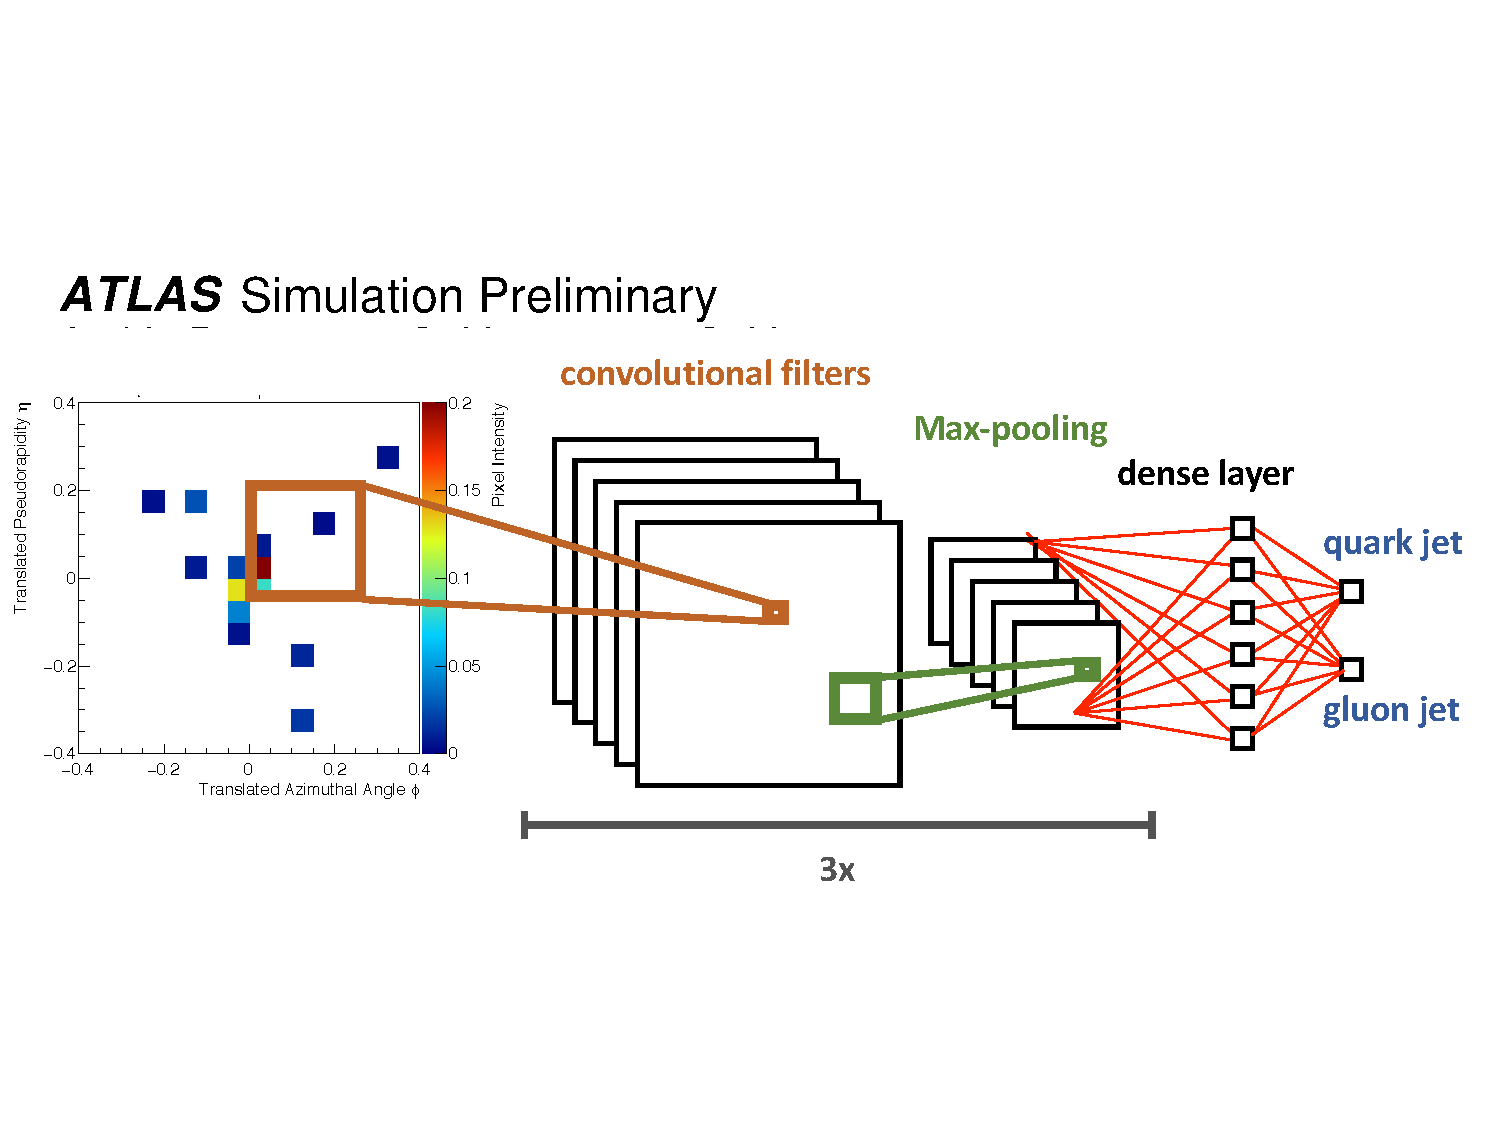
\includegraphics[width=0.8\textwidth]{figures/CNN/network.pdf}
\caption{Illustration of the deep convolutional neural network architecture.}
\label{fig:networkarch}
\end{center}
\end{figure}

Training is performed by minimizing the categorical crossentropy~\cite{Goodfellow-et-al-2016-Book}.
Minimization is performed with the Adam optimizer~\cite{DBLP:journals/corr/KingmaB14} 
as implemented in Keras~\cite{chollet2015keras} 
with a learning rate of 0.0001 over 50 iterations.
Training is performed using a single NVidia Tesla K80 GPU with 224000 jet images, while 56000 jet images are used for testing.
A typical training requires about 1 hour.
The network is retrained for each of the two $p_\text{T}$ ranges considered.

The output of the network corresponding to the quark jet class is used as a discriminant (\textit{CNN tagger}).
The discriminating power of the CNN tagger is compared with that of individual physically motivated observables, the calorimeter jet width $w$ and the number of tracks $n_\text{track}$, and their combination with the 2D binned likelihood ratio (LLH) in Figure~\ref{fig:classifiers}.  Simple thresholds are applied to construct the $n_\text{track}$ and jet width curves.  Interestingly, the CNN tagger has a similar performance to the classic $n_\text{track}$+jet width tagger that has been extensively studied in the past for quark versus gluon jet tagging~\cite{Aad:2014gea,ATLAS-CONF-2016-034}.  
The overall performance improves with $p_\text{T}$ as does the importance of $n_\text{track}$ relative to jet width since the number of particles inside quark and gluon jets increases with $p_\text{T}$.

%The CNN tagger outperforms the discrimination provided by the other discriminants across the full range of quark jet efficiency in both kinematic regimes considered, $150<\pt<200~\GeV$ and $400<\pt<500~\GeV$.

\begin{figure}[htpb]
\begin{center}
\subfloat[][]{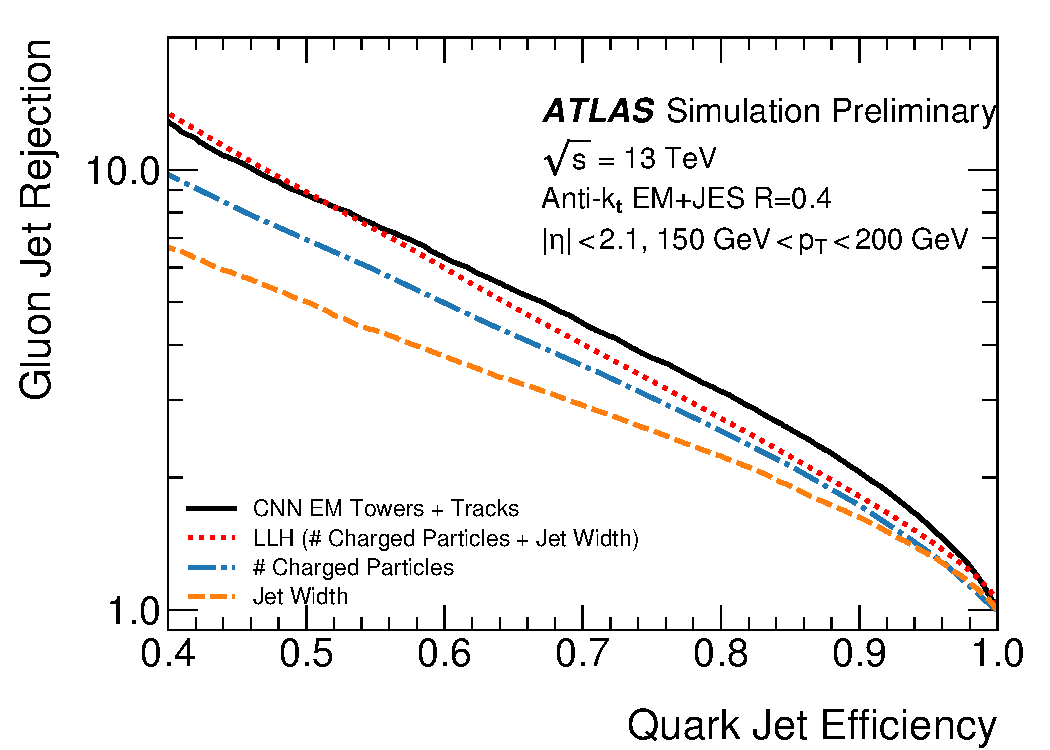
\includegraphics[width=0.5\textwidth]{figures/CNN/ROC_pt150_200_classifier.pdf}\label{lowpt}}
\subfloat[][]{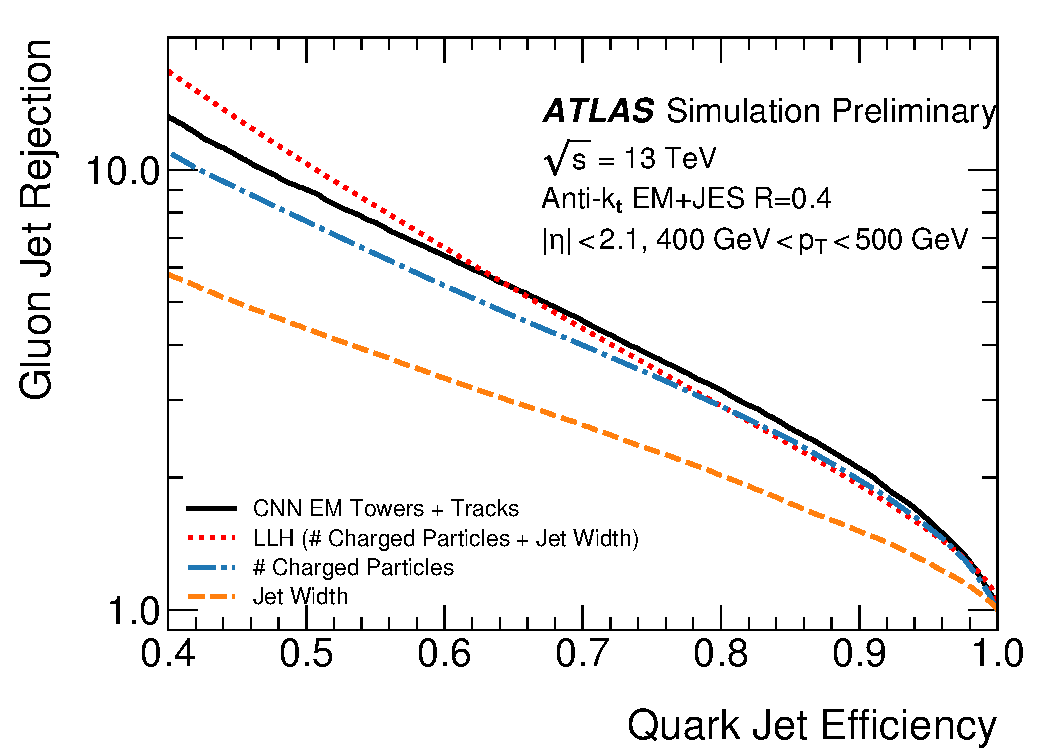
\includegraphics[width=0.5\textwidth]{figures/CNN/ROC_pt400_500_classifier.pdf}\label{highpt}}
\caption{Gluon jet rejection as a function of the quark jet efficiency using physics motivated observables and jet image discriminants
for jets with \protect\subref{lowpt} $150<\pt<200~\GeV$ and \protect\subref{highpt} $400<\pt<500~\GeV$.  The LLH is a tagger constructed from the optimal (likelihood) combination of $n_\text{track}$ and jet width. }
\label{fig:classifiers}
\end{center}
\end{figure}

Given the promising performance suggested by Fig.~\ref{fig:classifiers}, especially at lower $p_\text{T}$ and high efficiency, the remainder of this note is dedicated to a preliminary probe of where and how the CNN is able to distinguish quark and gluon jets based on their radiation pattern.


\clearpage

\subsection{Detector Regions}

Both tower and topocluster inputs are projected onto a regular grid, but variations in the underlying geometry of the calorimeter could have an impact on performance.  
Focusing on towers, Figure~\ref{fig:tracktruth}(b) shows that similar performance is achieved when testing the tagger on jets that are predominately in the barrel ($|\eta|<1.2$) 
to those that are in the transition region between the barrel and endcap calorimeters ($1.2<|\eta|<2.1$).
The full $|\eta|$ range ($|\eta|<2.1$) is used for training.


